\section{Experiments}
\label{sec:experiments}

This section describes our experiments we have specified and conducted to assess 
the behavior of 
our NDN model, under different cache algorithms. In 
Section~\ref{subsec:exp-setup}, we start 
with a brief description of the setup of our experiments, 
including the relevant parameters (e.g. number of content objects, popularity 
distribution, etc.), network topologies, cache characteristics, as well as the 
metrics to be considered. Later, in Section~\ref{subsec:exp-results}, we 
present the results of several experiment runs, according to the metrics 
specified in Section~\ref{subsec:exp-setup}.

\subsection{Experimental Setup}
\label{subsec:exp-setup}

The conducted experiments can be characterized along three main dimensions: (1) 
content object characteristics; (2) network topologies; and (3) cache 
characteristics.\shortvertbreak

\subsubsection{Content Object Characteristics}
\label{subsec:exp-setup-cobj}

For all experiments we consider a content object space of 
$|O| = 100$, with decreasing popularity and following a Zipf distribution: 
each content object $O_o$, with $o = \{1,2,...,|O|\}$, is requested by a client 
$C$ with probability $q_{o} = \frac{c}{o^{\alpha}}$, with $c = 0.8$ and 
$\alpha = \{0.5, 1, 2\}$.\shortvertbreak

At each experiment round (see Section~\ref{sec:impl} for more details on 
rounds), each client $C$ generates a signal for content object $O_o$ with 
probability $q_{o}$. We consider a number of rounds 
$|N| = 10000$ for all experiment runs.\shortvertbreak

\subsubsection{Network Topologies}
\label{subsec:exp-setup-nettop}

We consider two types of topologies: (1) a cascade topology with $|L| = 5$ levels 
($|C| = 1$, $|R| = 1$ and $|S| = 1$), shown in Figure~\ref{fig:exp-setup-nettop-cascade}; (2) a binary 
tree topology, also with $|L| = 5$ levels ($|C| = 8$, $|R| = 7$ and $|S| = 1$), as 
shown in Figure~\ref{fig:exp-setup-nettop-tree}. The definition of `level' is straightforward and depicted 
in Figure~\ref{fig:exp-setup-nettop}.\shortvertbreak

\begin{figure}[h!]
    \centering
    \subfigure[]{
        %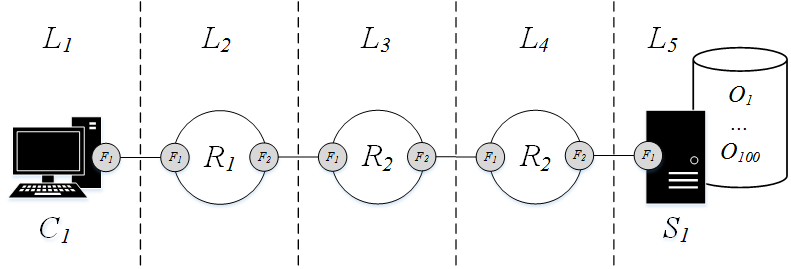
\includegraphics[width=0.40\textwidth] {figures/exp-setup-nettop-cascade.png}
        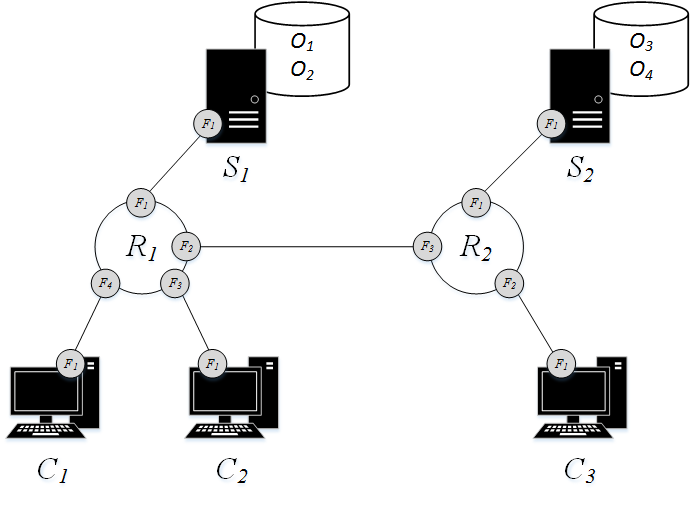
\includegraphics[width=0.30\textwidth] {figures/fib-topo.png}
        \label{fig:exp-setup-nettop-cascade}
    }

    \subfigure[]{
        %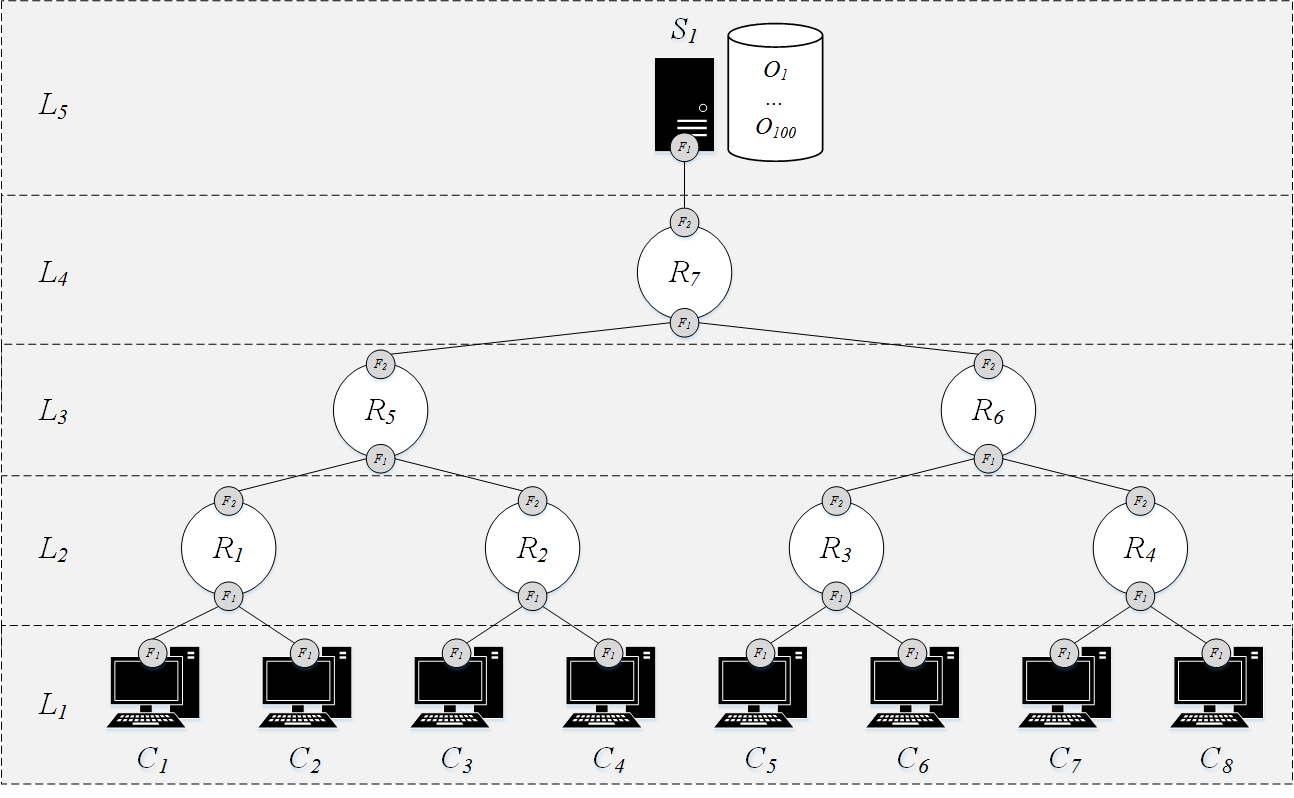
\includegraphics[width=0.40\textwidth] {figures/exp-setup-nettop-tree.png}
        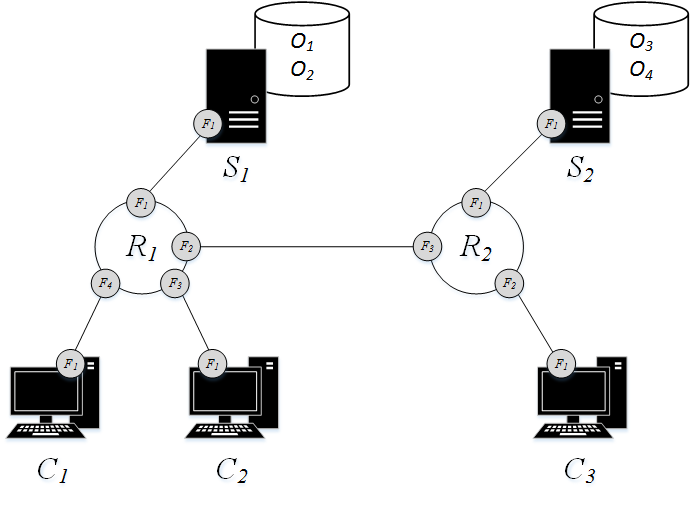
\includegraphics[width=0.30\textwidth] {figures/fib-topo.png}
        \label{fig:exp-setup-nettop-tree}
    }

    \cprotect\caption{Graphical depiction of the topologies considered for 
        our experiments: (a) cascade topology ($|L| = 5$, $|C| = 1$, $|R| = 1$ 
        and $|S| = 1$); (b) binary tree topology 
        ($|L| = 5$, $|C| = 8$, $|R| = 7$ and $|S| = 1$).}
    \label{fig:exp-setup-nettop}

\end{figure}

\subsubsection{Cache Characteristics}
\label{subsec:exp-setup-cache}

We evaluate the performance of our model under three different types of cache 
algorithms, already described in Section~\ref{subsec:meth-caching-algs}: (1) 
Least Recently Used (LRU); (2) More Recently Used (MRU); and (3) Random. We 
consider different cache sizes, specifically $|P| = \{10, 25, 50, 75\}$.\shortvertbreak

\subsubsection{Metrics}
\label{subsec:exp-setup-metrics}

For all our experiments we collect and evaluate the following metrics:

\begin{enumerate}

    \item Total number of Interests and Data packets received\slash sent per network node\slash level;
    \item Cache hit\slash miss rate per content object and network level;
    \item Number of Interest `hits', per content object and network level (including 
        server(s) $S$);
    \item Relative time spent at cache per content object.\shortvertbreak

\end{enumerate}

Regarding metric 2, we first provide our definition of `cache hit': a cache hit 
happens when an Interest signal for some content object $O_o$, arriving at some 
router $R_r$, finds a cached copy of $O_o$ at the CS of $R_r$. Therefore, to 
compute metric 2, we consider the Interest signals 
arriving at all NDN routers of some level $L$, discriminated by content 
object $O_o$, for all simulation rounds $N$. We then find the ratio between Interest 
`hits' for $O_o$, $i'_{O_o}$, and the total value of arriving Interests for $O_o$ at that 
level, $i_{O_o}$:

\begin{equation}
    \frac{\sum_{n=1}^{|N|} i'_{O_o}}{\sum_{n=1}^{|N|} i_{O_o}} \quad \forall \ R_r \ \text{in level $L$}
    \label{eq:exp-setup-metrics-2}
\end{equation}\shortvertbreak

For metric 4, we simply find the average number of rounds 
some content object $O_o$ spends at the caches of NDN routers of some level $L$, and find 
the ratio vs. the total number of simulation rounds.

\subsection{Experimental Results}
\label{subsec:exp-results}

\begin{figure}[h!]

    \centering
    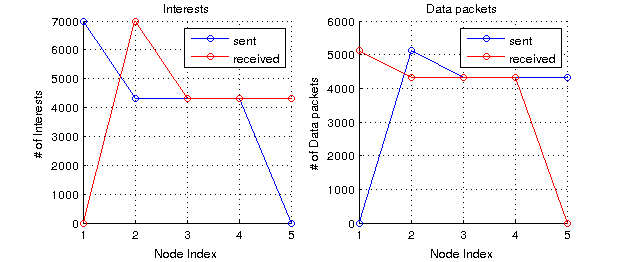
\includegraphics[width=0.50\textwidth]{figures/pre-test.png}
    \cprotect\caption{Graphical depiction of our NDN router model.}
    \label{fig:pre-test}

\end{figure}


